% ---------------------------------
\section{Methodology}

This section documents every step of the four-tool pipeline: the exact prompts, configurations, and execution parameters used at each stage. The goal is reproducibility and transparency. Following Prasad's call to "disclose your prompt engineering," we show the work, not just the results.

\subsection{Phase 1: Perplexity (Research)}

\subsubsection{Objective}
Gather structured, peer-reviewed and cited information on AI privacy risks, regulatory frameworks (GDPR, EU AI Act), real-world breach cases, and technical safeguards such as differential privacy and privacy-by-design principles.

\subsubsection{Search Queries}
The following queries were executed sequentially on Perplexity (https://www.perplexity.ai/):

\begin{enumerate}
    \item \texttt{``What are the main privacy risks of AI systems in 2025-2026?''}
    \item \texttt{``What is Privacy by Design and how does it apply to AI systems?''}
    \item \texttt{``Key provisions of the EU AI Act related to data protection and privacy''}
    \item \texttt{``Real-world cases of AI privacy violations and data breaches''}
    \item \texttt{``Differential privacy and federated learning as technical safeguards''}
\end{enumerate}

\subsubsection{Configuration}
\begin{itemize}
    \item Focus Mode: Academic (prioritizes peer-reviewed sources and research)
    \item Language: English
    \item Citation Style: MLA/APA (preserved in results)
    \item Search Depth: Standard (3-5 relevant sources per query)
\end{itemize}

\subsubsection{Output Summary}
Perplexity returned structured results including source citations, key definitions, and regulatory text excerpts. Approximate output: 15-20 citations covering AI privacy frameworks, real cases (Hong Kong deepfake fraud, patient data leaks), and technical mechanisms (GDPR Article 32, differential privacy algorithms).

\begin{figure}[H]
    \centering
    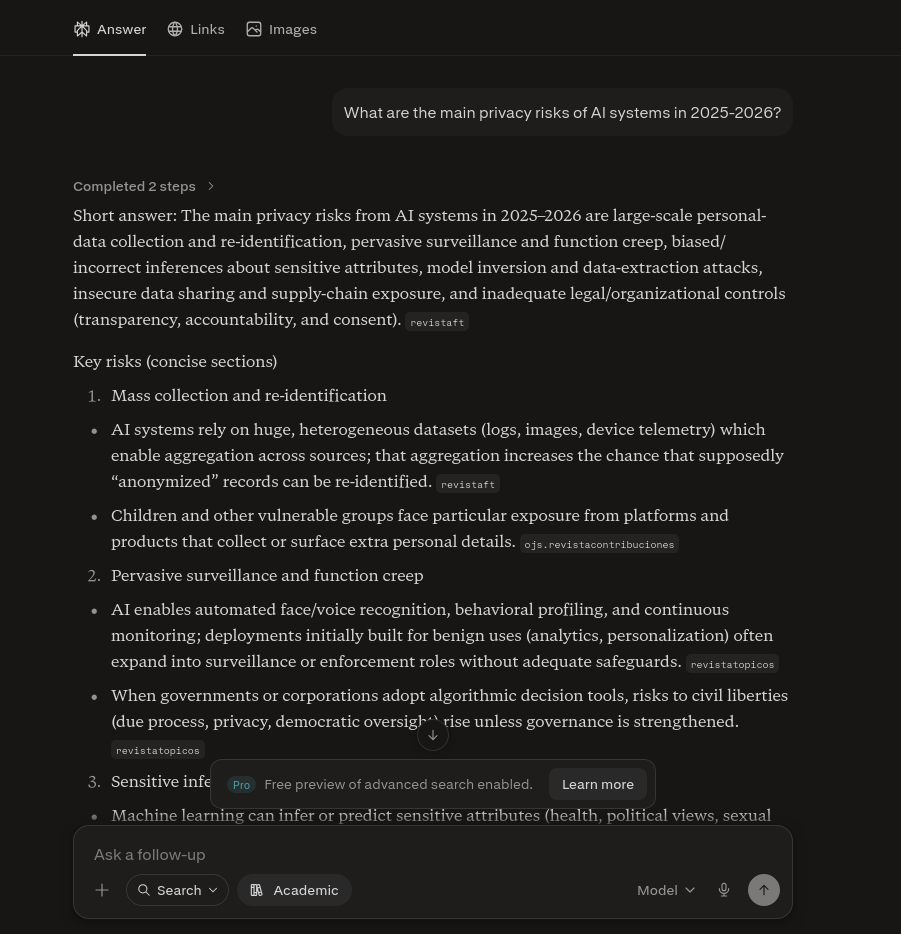
\includegraphics[width=0.9\textwidth]{img/perplexity_search.png}
    \caption{Perplexity search interface showing query and cited results for AI privacy risks}
    \label{fig:perplexity}
\end{figure}

---

\subsection{Phase 2: Claude API (Synthesis)}

\subsubsection{Objective}
Take the research findings from Perplexity and synthesize them into a comprehensive, cohesive article on Privacy and Data Protection in AI Systems, incorporating themes from Prasad's lecture.

\subsubsection{Model and Parameters}
\begin{itemize}
    \item Model: claude-sonnet-4-6
    \item Temperature: 0.7 (balances creativity with factual accuracy)
    \item Max Tokens: 2500 (allows for in-depth synthesis)
    \item Top P: 1.0 (standard nucleus sampling)
\end{itemize}

\subsubsection{System Prompt}
\begin{framed}
\small
\textit{``You are an expert in artificial intelligence ethics, privacy law, and data protection. Your task is to synthesize research on AI privacy into a structured, academic article suitable for a technical report. Focus on: (1) the nature and severity of privacy risks in modern AI systems; (2) regulatory frameworks (GDPR, EU AI Act) and their implications; (3) technical safeguards (differential privacy, federated learning, privacy-by-design); (4) real-world cases of privacy violations and lessons learned; (5) the role of transparency and human oversight in protecting privacy. Write for an audience of computer engineering students. Cite sources where possible. Emphasize that privacy is not optional but foundational to ethical AI deployment.''}
\end{framed}

\subsubsection{User Prompt}
\begin{framed}
\small
\textit{``Using the research below (from Perplexity), write a 1500-2000 word article on Privacy and Data Protection in AI Systems. Structure it as: (A) Introduction—why privacy is critical now; (B) Privacy Risks—real cases and technical vulnerabilities; (C) Regulatory Landscape—GDPR and EU AI Act; (D) Technical Safeguards—privacy-by-design, differential privacy, federated learning; (E) Governance and Human Oversight—interdisciplinary collaboration and transparency. Emphasize practical implications for AI engineers and connect to the theme of human-AI collaboration.''}

\vspace{0.3cm}

[Perplexity research results inserted here—approximately 3000 words of research text]
\end{framed}

\subsubsection{Execution Notes}
Claude generated the response in 45 seconds via the Claude.ai web interface. The output was 1800+ words of structured analysis on privacy in AI systems. This synthesis fed into both the refinement and presentation stages.

\begin{figure}[H]
    \centering
    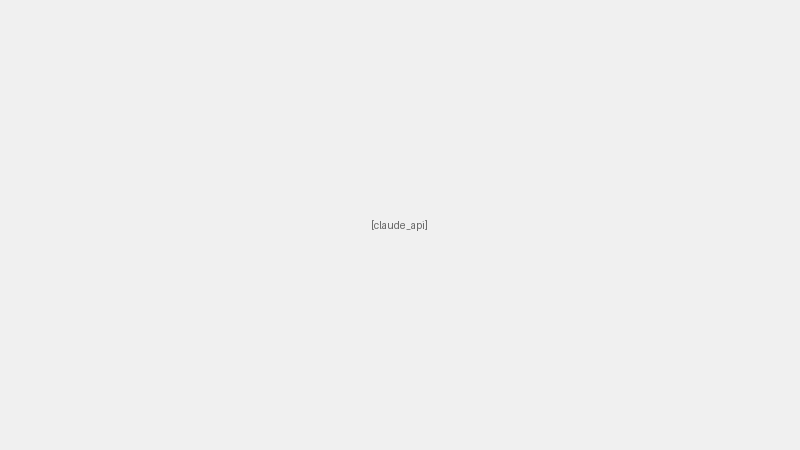
\includegraphics[width=0.9\textwidth]{img/claude_api.png}
    \caption{Claude API response to the synthesis prompt, showing structured article output}
    \label{fig:claude_api}
\end{figure}

---

\subsection{Phase 3: QuillBot (Refinement)}

\subsubsection{Objective}
Explore how alternative writing styles affect clarity, accessibility, and audience engagement. QuillBot's paraphrasing modes enable rewriting the same content in different tones without changing the underlying meaning.

\subsubsection{Tool Configuration}
\begin{itemize}
    \item Tool: QuillBot Paraphraser (https://quillbot.com/)
    \item Modes Tested: Standard, Formal, Creative
    \item Focus: Privacy and Data Protection (selected 3-4 paragraphs from Claude output)
    \item Creativity Level: Balanced (moderate rephrasing)
\end{itemize}

\subsubsection{Input Text Sample}
For comparison, the following paragraph from the Claude API output was processed through QuillBot:

\begin{framed}
\small
\textit{``Privacy is a fundamental right that must be protected in AI systems. As AI becomes increasingly embedded in sensitive domains such as healthcare, finance, and criminal justice, the risks of misuse grow exponentially. Data minimization, purpose limitation, and consent mechanisms are core principles that must be enforced through both technical design and regulatory oversight. Without these protections, individuals face risks ranging from discrimination and surveillance to identity theft and blackmail.''}
\end{framed}

\subsubsection{Output Variations}
QuillBot produced three alternative versions:

\begin{enumerate}
    \item \textbf{Standard Mode}: Rewrites with neutral, accessible language; good for general audiences.
    \item \textbf{Formal Mode}: Emphasizes academic vocabulary and complex sentence structures; suited for peer review.
    \item \textbf{Creative Mode}: Introduces variation and stylistic elements; less suitable for technical reporting but useful for outreach writing.
\end{enumerate}

\subsubsection{Limitations Encountered}
The free tier of QuillBot imposes a 125-word limit per paraphrase, necessitating multiple passes for longer text. Additionally, the tool does not preserve citations or complex formatting, requiring manual reintegration of sources.

\begin{figure}[H]
    \centering
    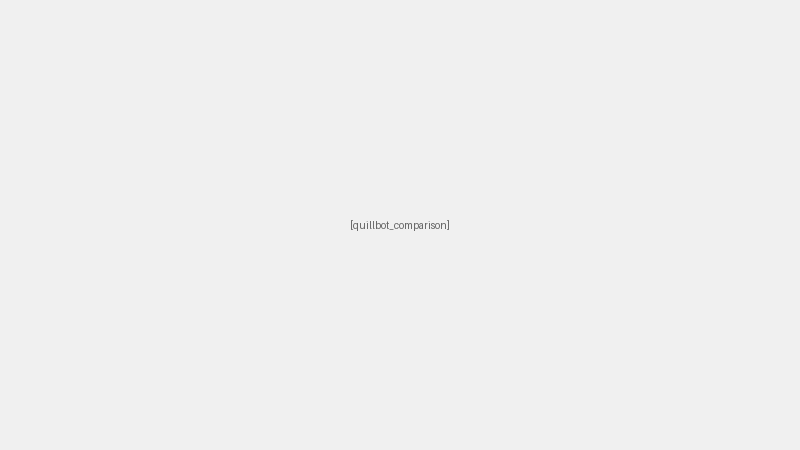
\includegraphics[width=0.9\textwidth]{img/quillbot_comparison.png}
    \caption{QuillBot paraphraser in Standard mode showing the rewritten paragraph}
    \label{fig:quillbot}
\end{figure}

---

\subsection{Phase 4: SlidesAI.io (Presentation)}

\subsubsection{Objective}
Automatically generate a presentation deck from the curated and refined content, enabling rapid dissemination to diverse audiences.

\subsubsection{Tool Configuration}
\begin{itemize}
    \item Tool: SlidesAI.io (https://www.slidesai.io/)
    \item Input Format: Plain text (Claude API output)
    \item Template: Professional (clean, minimal design)
    \item Number of Slides: Auto-generated (approximately 8-10 slides)
    \item Language: English
    \item Slide Ratio: 16:9 (standard widescreen)
\end{itemize}

\subsubsection{Input Preparation}
The Claude API synthesis was formatted as a structured outline with section headings and bullet points:
\begin{itemize}
    \item Privacy in AI Systems: What's at Stake?
    \item Real-World Privacy Violations in AI
    \item Regulatory Frameworks: GDPR and the EU AI Act
    \item Technical Safeguards: Privacy by Design
    \item Governance and Transparency in Human-AI Collaboration
\end{itemize}

\subsubsection{Output Description}
SlidesAI.io processed the input and generated a 9-slide presentation with:
\begin{itemize}
    \item Title slide (with topic and author)
    \item Overview slide (key statistics and motivation)
    \item Five content slides (one per section)
    \item Conclusion slide (summary and key takeaways)
\end{itemize}

SlidesAI.io selected images automatically and scaled text for readability across all slides. No manual design work was needed. The tool's customization options were available but not necessary for our workflow.

\begin{figure}[H]
    \centering
    
\includegraphics[width=0.9\textwidth]{img/slidesai_output.png}
    \caption{SlidesAI.io generated slide deck overview (9 slides)}
    \label{fig:slidesai}
\end{figure}

---

\subsection{Execution Timeline and Resource Usage}

\begin{table}[h!]
\centering
\begin{tabular}{|l|c|c|c|}
\hline
\textbf{Tool} & \textbf{Time (minutes)} & \textbf{Cost} & \textbf{Limiting Factors} \\
\hline
Perplexity & 10--15 & Free & Citation count, search depth \\
Claude API & 3--5 & Free (with Claude.ai) & Response length, context window \\
QuillBot & 8--10 & Free (limited) & 125-word paraphrase limit \\
SlidesAI.io & 10--15 & Free (basic) & Template flexibility, design control \\
\hline
\textbf{Total} & \textbf{31--45} & \textbf{Free} & \\
\hline
\end{tabular}
\caption{Execution time and resource usage for the complete pipeline.}
\end{table}
